\chapter{\label{sec:design}Design}

%trusted execution through openness, crowdsourcing, and voting (e.g. Ethereum VM)
%NodeJS == social trust
%Github == social
%Solidity == ?
%Event-based architecture
%Internet-based (live overlay)
%any-platform (even including Android, GUI framework; thus only common denominator: HTML)
%network availability
%module identifier promotes trust
%Voting
%double vote detection by checking the blockchain
%Modules search for dependencies downwards
%View layer triggers search for logic layer
%Logic layer triggers search for other logic layer
%After search they register with the higher module
%Module abstracts classes for registration mechanism
%Module distribution mechanism
%Send message to all neighbours when voting
%Send message to random neighbour every x time units to keep modules circulating
%Random sending based on votes, lifetime, reputation
%Each nodes downloads module to increase availability in the network
%After x time units unused/unstored modules get deleted
%Mention malicious nodes
%Track of module is used to determine if it can be deleted
%Find different module versions by module identifier
%crawl neighbour nodes
%Modules
%Modules should have votes per version to prevent major code changes
%Code should be viewable
%Version number is hash code to prevent version tempering
%Each module has own pub key for identifier
%Decide to keep author in module identifier
%Decide if each version should be a separate module, has downsides to upgrade speed
%Key value store for storing settings in dependent modules
%Execution
%Docker runner
%Local runner

% code review, trust, untrusted code execution, dynamic module loading, dependencies loading

This chapter will expand on the design of the proposed framework. It will elaborate on the high-level structures within the application. The implementation considerations and details will be discussed in Chapter~\ref{sec:implementation}. The evaluation of the framework through an experiment will be  done in Chapter~\ref{sec:experimentation-and-evaluation}.

\section{Overview}

An overview of the architecture of the framework can be found in Figure~\ref{fig:architecture}. It shows the three different layers that make up the framework. These layers are connected by a system-wide event bus that is used for connecting different parts of the application to each other.

These layers together create the components needed to run and distribute modularized code in a distributed fashion. The next few sections will expand on each of the mentioned layers and their components.

% Expand on concept

\begin{figure}[h]
	\centering
	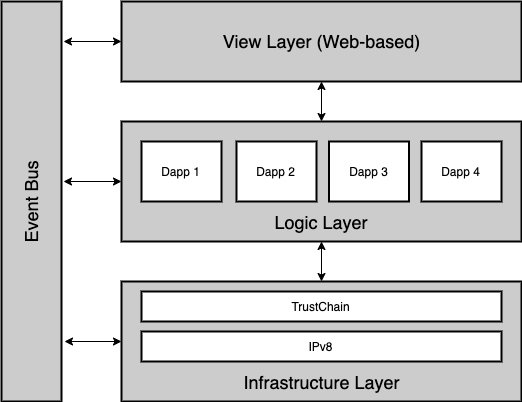
\includegraphics[width=0.5\textwidth]{images/architecture.png}
	\caption{\label{fig:architecture}}
\end{figure}

\section{Event-driven Architecture}

% event-driven architecture (event bus)

The framework is designed for running many different isolated applications. These applications consist out of separate modularized components that each run on different layers. Connecting these components together to form the application can quickly become a mess. To prevent this from happening, the framework makes use of an event-driven architecture. In such an architecture, actions are taken based on other actions happening in the system. Creating simple and maintainable logic. Input such as human interaction, network packets, creation of components, and/or system events, trigger corresponding actions in other parts of the system. An example of this would be the downloading of a module when a new one is discovered. This event system is located in the infrastructure layer and communicates with the other layers through the event bus. This event bus allows other parts of the system to hook on to specific events triggered by certain actions. To allow components to hook onto such an event they have to register an event handler with the event bus for the types of events it wants to act on.

\section{View Layer}

% view layer interface (events, rest endpoint)

The view layer contains the components that deal with human interaction. These components consist out of user interfaces created using web technologies. The decision for using web-based user interface was made because it is the current day standard for making cross-platform compatible GUIs and it allows for easy decoupling between itself and the logic behind it.

A view layer component consists out of a HTML, CSS, and javascript website. This website is run as a standalone component and connects to its logic counterpart through a REST API. This decouples the user interface part of the application and allows it to be interchanged. Multiple different GUIs could be offered for the same application.

When a new view component is added to the system, it needs to know how to connect to the logic component of the application. It does this by triggering an event on the event bus, specific for the type of application it belongs to, indicating it is requesting an endpoint address. The logic component is subscribed to this event. Its registered handler will return the REST API endpoint address back to the view component through the event bus.

To define a view component, a special file has to be created: view-component.json. This definition file stores the attributes and the settings of the view component. Attributes of the file include: name, version, app-tag (Application tag used for hooking on to the logic component). Each view component also needs to have a directory named public which contains the index.html file. An example structure can be found below.

\begin{itemize}
	\item view-component.json
	\item public \begin{itemize}
		\item index.html
		\item Other HTML/CSS/javascript resources
	\end{itemize}
\end{itemize}

% Component definition: component.json, properties, directory structure

\section{Logic Layer}

% logic layer (dapps, dapp interface, types of dapps, dapp definition language, versioning, states, live re-loading, caching strategies, identity profiles (anonymous, shared identities), isolation)

The logic layer contains the components that deal with the functionality of the application. Each component is defined by a file called: component.json located in the root of the component's directory. This file stores the properties and the settings of the logic component. The default properties that need to be defined are: name, version, app-tag, type. The component can be one of three types: Code, Overlay, or Service

\subsection{Code Component}

The code component consists out of a Python script without decentralized functionality that is executed on the host system. These types of components can be used as simple code scripts or as building blocks for bigger and more complex components. An example of this would be an updater script or an interface implementation.

In addition to the default properties a logic component defines, the code component also defines a function that needs to be executed when the module is run.

\subsection{Overlay Component}

The overlay component consists out of a decentralized overlay built on the IPv8 network. This component requires all files necessary to run an IPv8 overlay. This type of component runs in a shared environment and can have access to other overlay components in this same environment.

In addition to the default properties a logic component defines, the overlay component also defines the overlay class and overlay settings

% specific component properties

\subsection{Service Component}

The service component consists out of a twisted service. This service type can be used to run processes in the background or isolate certain processes from other processes in the system.

In addition to the default properties a logic component defines, the service component also defines the service class.

% specific component properties

\subsection{Versioning}

A system without versioning can quickly become infected and would make it difficult to track on which iteration the system is running. That is why each component has a component name and a version. The name property is a unique value for each component used to differentiate it from other components. The version property is value that is incremented every time a change has been made to the component. Together these properties form the identifier of the component.

\section{Infrastructure Layer}

infrastructure layer is responsible for providing network functionality and lower level functionality like storage. It accomplishes this through multiple different modules. Twisted is responsible for allowing pseudo multi threading through event-driven architecture. IPv8 is responsible for providing overlay functionality to run decentralized applications in and on the framework. TrustChain is responsible for providing a decentralized blockchain storage. LibTorrent is responsible for providing file transport services.

\section{Identity Profiles}

In peer-to-peer systems each peer in an overlay has to have an identity. This identity determines the trust and association within and across overlays. This identity can be shared between different overlays or each overlay can use its own identity. If two overlays use the same identity, one overlay can benefit from the built up trust and reputation of another overlay. However, actions performed by one overlay can also have a negative trust impact on the other overlay. To allow applications to choose between the having a shared identity, having its own identity, or having an pseudo-random identity,  the framework provides a configuration option in the component.json to select what kind of identity profile is preferred..  

\section{System Strategies}

Since the framework deals with untrusted executable user code, the framework provides several different strategies that the user can select from to protect their system against possible threats from running this code.

\subsection{Download and Retention Strategy}

The framework allows the user to configure and replace the download and retention strategy. This strategy is responsible for choosing which components get downloaded and how long they are kept on the system. For the distribution of components it is necessary to download packages that might not be used by the host system itself, but are solely for the intent of distributing. Some users might want to take a different approach to accomplish this. The framework addresses this by allowing parts of its code to be replaced by other components written by a third-part or by the user itself.

\subsection{Isolated Execution}

Since all distributed components have to be executed on the host system for them to function, it can pose a security risk by running untrusted user code. To minimize the risk that this poses, the framework allows components to be run inside of an isolated execution environment using Docker. When this method is used an execution environment is setup inside of the docker engine and the code will be mounted inside of this container. This container will then be able to run the code in isolation. This method, however, will prevent other applications running on the system from communication to it. It does allow the view layer to communicate with the isolated components since this makes use of network sockets.

% infrastructure layer (TrustChain, IPv8, DB, LibTorrent, caching) 